\newpage
\section{Phân loại thư rác trên tập dữ liệu Enron-Spam}

\subsection{Tổng quan}
\paragraph{}{Bộ dữ liệu \textbf{Enron-Spam} là một nguồn tài liệu tuyệt vời được thu thập bởi V. Metsis, I. Androutsopoulos và G. Paliouras và được mô tả trong ấn phẩm của họ "Spam Filtering with Naive Bayes - Which Naive Bayes?" \cite{metsis2006spam}. Bộ dữ liệu chứa tổng cộng 17.171 thư rác và
16.545 thư không phải thư rác ("ham") (tổng cộng 33.716 thư điện tử).}

\paragraph{}{Dựa trên kiến thức lý thuyết về Maximum Likelihood Estimation (MLE), Maximum A Posteriori Estimation (MAP) và mô hình Bag-of-Words, chúng tôi sẽ sử dụng mô hình thống kê \textbf{Naive Bayes Classifier} để \textbf{phân loại thư rác} trên bộ dữ liệu Enron-Spam. Quy trình các bước như sau:}

\begin{enumerate}
    \item \textbf{Tải, khám phá và tiền xử lý dữ liệu.}
    \item \textbf{Vector hóa văn bản dựa trên mô hình Bag-of-Words.}
    \item \textbf{Phân loại thư rác bằng Multinomial Naive Bayes.}
    \item \textbf{Đánh giá mô hình bằng độ chính xác, ma trận nhầm lẫn.}
\end{enumerate}

\subsection{Bộ dữ liệu Enron-Spam và tiền xử lý dữ liệu}
\paragraph{}{Bộ dữ liệu \textbf{Enron-Spam} được cung cấp dưới dạng 2 file: \texttt{train.csv} và \texttt{val.csv},  ứng với 2 tập \textbf{training} và \textbf{validation}. Trong đó gồm: 
\begin{itemize}
    \item \texttt{train.csv}: 27284 dòng; 4 cột: \texttt{Message ID}, \texttt{Subject}, \texttt{Message}, \texttt{Spam/Ham}.
    \item \texttt{val.csv}: 3084 dòng; 4 cột: \texttt{Message ID}, \texttt{Subject}, \texttt{Message}, \texttt{Spam/Ham}.
    \begin{itemize}
        \item \texttt{Message ID}: Chỉ số của thư.
        \item \texttt{Subject}: Tiêu đề thư
        \item \texttt{Message}: Nội dung thư.
        \item \texttt{Spam/Ham}: Biến phân loại thư. \texttt{Ham} là thư bình thường, \texttt{Spam} là thư rác.
    \end{itemize}
\end{itemize}

Đây lần lượt là 5 dòng đầu tiên của tập training (\texttt{train.csv}) và tập validation (\texttt{val.csv}):

\begin{figure}[H]
    \centering
    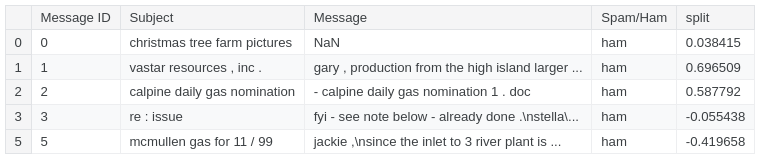
\includegraphics[width=1\linewidth]{img/05-dftrain-head.png}
    \caption{5 dòng đầu tiên của tập train}
\end{figure}

\begin{figure}[H]
    \centering
    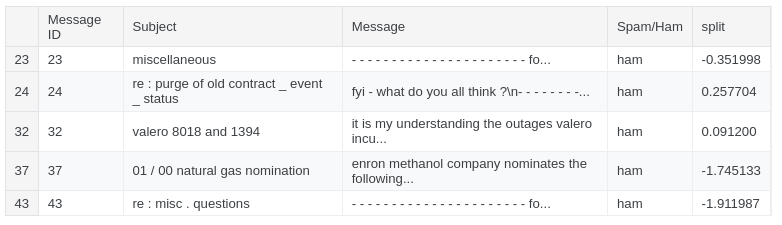
\includegraphics[width=1\linewidth]{img/05-dfval-head.png}
    \caption{5 dòng đầu tiên của tập validation}
\end{figure}

\paragraph{}{Với các bước tiền xử lý dữ liệu, chúng tôi lần lượt áp dụng các kĩ thuật sau:}

\begin{enumerate}
    \item \textbf{Thay thế các ô NaN} (Not-a-Number) bằng chuỗi kí tự rỗng. Chuyển các kí tự chữ thành chữ thường.
    \item \textbf{Gộp chuỗi kí tự} trong hai cột \texttt{Subject} và \texttt{Message} thành một chuỗi kí tự duy nhất và tạo cột mới: \texttt{full\_text}.
    \item \textbf{Chuyển đổi nhãn} của cột \texttt{ham/spam} thành số: \texttt{ham -> 0}, \texttt{spam -> 1}.
\end{enumerate}

\subsection{Vector hóa văn bản bằng Bag-of-Words}

\paragraph{}{Chúng tôi áp dụng phương pháp Bag-of-Words được nhắc đến trong phần \ref{bow-section} để chuyển đổi các chuỗi kí tự trong cột \texttt{full\_text} (được hợp bởi \texttt{Subject} và \texttt{Message}) thành vector. Các vector này có đặc điểm:}

\begin{itemize}
    \item Mỗi vector ứng với một \texttt{full\_text} của một thư. Các vector này biểu diễn tần suất xuất hiện của các từ có trong \texttt{full\_text}.
    \item Kích thước các vector là bằng nhau và bằng với số lượng từ của từ điển được xây dựng trên toàn bộ cột \texttt{full\_text}, theo phương pháp Bag-of-Words.
    \item Mỗi vector có kích thước là \texttt{(1, 37830)}, ứng với số lượng từ có trong từ điển là 37830.
\end{itemize}

\subsection{Multinomial Naive Bayes}
\paragraph{}{Mô hình được sử dụng trong quá trình huấn luyện là \textbf{Multinomial Naive Bayes}, một mô hình xác suất dựa trên \textit{định lý Bayes} với giả định ``naive'' rằng các đặc trưng là \textit{độc lập có điều kiện} khi biết nhãn lớp. Đây là lựa chọn đặc biệt phù hợp trong các bài toán phân loại văn bản, nơi mà đặc trưng của dữ liệu là \textit{tần suất xuất hiện của từ} trong tài liệu.}

\subsubsection{Huấn luyện mô hình (fit)}

\textbf{Mục tiêu:} Học các tham số của mô hình từ tập dữ liệu huấn luyện.

\textbf{Quy trình huấn luyện:}
\begin{enumerate}
    \item \textbf{Xây dựng từ điển}: Thu thập tất cả các từ xuất hiện trong tập dữ liệu huấn luyện để tạo không gian đặc trưng.
    \item \textbf{Vector hóa dữ liệu}: Biểu diễn các văn bản dưới dạng ma trận BoW (\textit{Bag-of-Words}).
    \item \textbf{Tính log xác suất tiên nghiệm $P(c)$}:
    \[
    P(c) = \frac{N_c}{N}
    \]
    trong đó $N_c$ là số lượng mẫu thuộc lớp $c$, và $N$ là tổng số mẫu trong tập huấn luyện.
    \item \textbf{Tính tổng số từ xuất hiện trong mỗi lớp}.
    \item \textbf{Tính log xác suất có điều kiện (likelihood)} $P(\text{word}_i \mid c)$ cho mỗi từ và mỗi lớp.
\end{enumerate}

\subsubsection{Dự đoán log xác suất hậu nghiệm cho một vector BoW thưa}

\textbf{Mục tiêu:} Tính toán \textit{log của tử số xác suất hậu nghiệm} cho một văn bản (biểu diễn dưới dạng vector BoW thưa) tương ứng với từng lớp.

Với mỗi văn bản $x^{(i)}$, mô hình tính:
\[
\log P(c) + \sum_{j} x^{(i)}_j \cdot \log P(\text{word}_j \mid c)
\]
trong đó $x^{(i)}_j$ là số lần từ thứ $j$ xuất hiện trong văn bản $x^{(i)}$.

Không áp dụng phép chuẩn hoá (tức không chia cho mẫu số), vì ta chỉ cần so sánh tương đối giữa các lớp.

Nhãn dự đoán $\hat{y}^{(i)}$ được xác định theo nguyên lý \textbf{Maximum A Posteriori (MAP)}:
\[
\hat{y}^{(i)} = \arg\max_{c \in \mathcal{C}} \left( \log P(c) + \sum_{j} x^{(i)}_j \cdot \log P(\text{word}_j \mid c) \right)
\]

Quá trình này được áp dụng cho mọi $i = 1, \ldots, n$, tạo thành vector dự đoán:
\[
\hat{y} = [\hat{y}^{(1)}, \hat{y}^{(2)}, \ldots, \hat{y}^{(n)}]
\]

\subsection{Đánh giá mô hình}

\paragraph{}{Ở bước đánh giá mô hình, chúng tôi sử dụng 2 phương pháp chính là \textbf{độ chính xác} (accuracy) và \textbf{ma trận nhầm lẫn} (confusion matrix).}
\begin{itemize}
    \item \textbf{Độ chính xác:} Được tính bằng số trường hợp mô hình phân loại \texttt{ham/spam} đúng trên tổng số trường hợp cần phân loại.
    \item \textbf{Ma trận nhầm lẫn}: Phương pháp đánh giá hiệu suất của bài toán phân loại, trong đó:
    \begin{itemize}
        \item TP (True Positive): Số lượng thư \texttt{spam} được phân loại đúng. 
        \item TN (True Negative): Số lượng thư \texttt{ham} được phân loại đúng. 
        \item FP (False Positive - Type 1 Error): Số lượng thư \texttt{ham} bị phân loại sai thành \texttt{spam}. 
        \item FN (False Negative - Type 2 Error): Số lượng thư \texttt{spam} bị phân loại sai thành \texttt{ham}. 
    \end{itemize}
\end{itemize}

\begin{figure}[H] 
    \centering 

    \begin{subfigure}[b]{0.48\textwidth} 
        \centering
        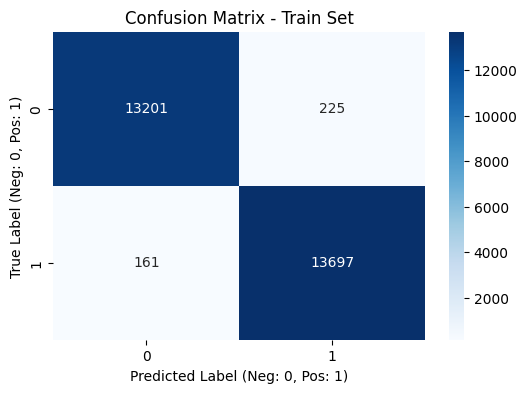
\includegraphics[width=\linewidth]{img/confusion_matrix_train_set.png}
        \caption{Độ chính xác trên tập Training: 0.9893}
        \label{fig:training_results}
    \end{subfigure}
    \hfill 
    \begin{subfigure}[b]{0.48\textwidth} 
        \centering
        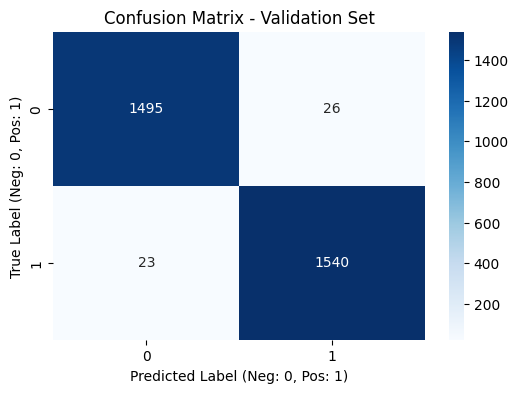
\includegraphics[width=\linewidth]{img/confusion_matrix_valid_set.png}
        \caption{Độ chính xác trên tập Validation: 0.9857}
        \label{fig:validation_results}
    \end{subfigure}

    \caption{Ma trận nhầm lẫn của mô hình trên tập training và validation} 
    \label{fig:overall_results}
\end{figure}